% \chapter{Pokyny a návody k formátování textu práce}
% \textbf{\large Tato příloha samozřejmě nebude součástí vaší práce. Slouží pouze jako příklad formátování textu.}
% 
% Používat se dají všechny příkazy systému \LaTeX. Existuje velké množství volně přístupné dokumentace, tutoriálů, příruček a dalších materiálů v elektronické podobě. Výchozím bodem, kromě Googlu, může být stránka CSTUG (Czech Tech Users Group) \cite{CSTUG}. Tam najdete odkazy na další materiály.  Vetšinou dostačující a přehledně organizovanou elektronikou dokumentaci najdete například na \cite{latexdocweb} nebo \cite{latexwiki}.
% 
% Existují i různé nadstavby nad systémy \TeX{} a \LaTeX, které výrazně usnadní psaní textu zejména začátečníkům. Velmi rozšířený v Linuxovém prostředí je systém Kile.
% 
% 
% \section{Vkládání obrázků}
% Obrázky se umísťují do plovoucího prostředí \verb|figure|. Každý obrázek by měl obsahovat \textbf{název} (\verb|\caption|) a \textbf{návěští} (\verb|\label|). Použití příkazu pro vložení obrázku \\\verb|\includegraphics| je podmíněno aktivací (načtením) balíku graphicx příkazem\\ \verb|\usepackage{graphicx}|.
% 
% Budete-li zdrojový text zpracovávat pomocí programu \verb|pdflatex|, očekávají se obrázky s příponou \verb|*.pdf|\footnote{pdflatex umí také formáty PNG a JPG.}, použijete-li k formátování \verb|latex|, očekávají se obrázky s příponou \verb|*.eps|.\footnote{Vzájemnou konverzi mezi snad všemi typy obrazku včetně změn vekostí a dalších vymožeností vám může zajistit balík ImageMagic  (http://www.imagemagick.org/script/index.php). Je dostupný pod Linuxem, Mac OS i MS Windows. Důležité jsou zejména příkazy convert a identify.}
% 
% \begin{figure}[ht]
% \begin{center}
% \includegraphics[width=5cm]{figures/LogoCVUT}
% \caption{Popiska obrázku}
% \label{fig:logo}
% \end{center}
% \end{figure}
% 
% Příklad vložení obrázku:
% \begin{verbatim}
% \begin{figure}[h]
% \begin{center}
% \includegraphics[width=5cm]{figures/LogoCVUT}
% \caption{Popiska obrazku}
% \label{fig:logo}
% \end{center}
% \end{figure}
% \end{verbatim}
% 
% \section{Kreslení obrázků}
% Zřejmě každý z vás má nějaký oblíbený nástroj pro tvorbu obrázků. Jde jen o to, abyste dokázali obrázek uložit v požadovaném formátu nebo jej do něj konvertovat (viz předchozí kapitola). Je zřejmě vhodné kreslit obrázky vektorově. Celkem oblíbený, na ovládání celkem jednoduchý a přitom dostatečně mocný je například program Inkscape.
% 
% Zde stojí za to upozornit na kreslící programe Ipe \cite{ipe}, který dokáže do obrázku vkládat komentáře přímo v latexovském formátu (vzroce, stejné fonty atd.). Podobné věci umí na Linuxové platformě nástroj Xfig. 
% 
% Za pozornost ještě stojí schopnost editoru Ipe importovat obrázek (jpg nebo bitmap) a krelit do něj latexovské popisky a komentáře. Výsledek pak umí exportovat přímo do pdf.
% 
% \section{Tabulky}
% Existuje více způsobů, jak sázet tabulky. Například je možno použít prostředí \verb|table|, které je velmi podobné prostředí \verb|figure|. 
% 
% \begin{table}
% \begin{center}
% \begin{tabular}{|c|l|l|}
% \hline
% \textbf{DTD} & \textbf{construction} & \textbf{elimination} \\
% \hline
% $\mid$ & \verb+in1|A|B a:sum A B+ & \verb+case([_:A]a)([_:B]a)ab:A+\\
% &\verb+in1|A|B b:sum A B+ & \verb+case([_:A]b)([_:B]b)ba:B+\\
% \hline
% $+$&\verb+do_reg:A -> reg A+&\verb+undo_reg:reg A -> A+\\
% \hline
% $*,?$& the same like $\mid$ and $+$ & the same like $\mid$ and $+$\\
% & with \verb+emtpy_el:empty+ & with \verb+emtpy_el:empty+\\
% \hline
% R(a,b) & \verb+make_R:A->B->R+ & \verb+a: R -> A+\\
%  & & \verb+b: R -> B+\\
% \hline
% \end{tabular}
% \end{center}
% \caption{Ukázka tabulky}
% \label{tab:tab1}
% \end{table}
% 
% Zdrojový text tabulky \ref{tab:tab1} vypadá takto:
% \begin{verbatim}
% \begin{table}
% \begin{center}
% \begin{tabular}{|c|l|l|}
% \hline
% \textbf{DTD} & \textbf{construction} & \textbf{elimination} \\
% \hline
% $\mid$ & \verb+in1|A|B a:sum A B+ & \verb+case([_:A]a)([_:B]a)ab:A+\\
% &\verb+in1|A|B b:sum A B+ & \verb+case([_:A]b)([_:B]b)ba:B+\\
% \hline
% $+$&\verb+do_reg:A -> reg A+&\verb+undo_reg:reg A -> A+\\
% \hline
% $*,?$& the same like $\mid$ and $+$ & the same like $\mid$ and $+$\\
% & with \verb+emtpy_el:empty+ & with \verb+emtpy_el:empty+\\
% \hline
% R(a,b) & \verb+make_R:A->B->R+ & \verb+a: R -> A+\\
%  & & \verb+b: R -> B+\\
% \hline
% \end{tabular}
% \end{center}
% \caption{Ukázka tabulky}
% \label{tab:tab1}
% \end{table}
% \begin{table}
% \end{verbatim}
% 
% \section{Odkazy v textu}
% \subsection{Odkazy na literaturu}
% Jsou realizovány příkazem \verb|\cite{odkaz}|. 
% 
% Seznam literatury je dobré zapsat do samostatného souboru a ten pak zpracovat programem bibtex (viz soubor \verb|reference.bib|). Zdrojový soubor pro \verb|bibtex| vypadá například takto:
% \begin{verbatim}
% @Article{Chen01,
%   author  = "Yong-Sheng Chen and Yi-Ping Hung and Chiou-Shann Fuh",
%   title   = "Fast Block Matching Algorithm Based on 
%              the Winner-Update Strategy",
%   journal = "IEEE Transactions On Image Processing",
%   pages   = "1212--1222",
%   volume  =  10,
%   number  =   8,
%   year    = 2001,
% }
% 
% @Misc{latexdocweb,
%   author  = "",
%   title   = "{\LaTeX} --- online manuál",
%   note    = "\verb|http://www.cstug.cz/latex/lm/frames.html|",
%   year    = "",
% }
% ...
% \end{verbatim}
% 
% %11.12.2008, 3.5.2009
% \textbf{Pozor:} Sazba názvů odkazů je dána Bib\TeX{} stylem\\ (\verb|\bibliographystyle{abbrv}|). 
% %Budete-li používat české prostředí (\verb|\usepackage[czech]{babel}|), 
% Bib\TeX{} tedy obvykle vysází velké pouze počáteční písmeno z názvu zdroje, 
% ostatní písmena zůstanou malá bez ohledu na to, jak je napíšete. 
% Přesněji řečeno, styl může zvolit pro každý typ publikace jiné konverze. 
% Pro časopisecké články třeba výše uvedené, jiné pro monografie (u nich často bývá 
% naopak velikost písmen zachována).
% 
% Pokud chcete Bib\TeX u napovědět, která písmena nechat bez konverzí 
% (viz \texttt{title = "\{$\backslash$LaTeX\} -{}-{}- online manuál"} 
% v~předchozím příkladu), je nutné příslušné písmeno (zde celé makro) uzavřít 
% do složených závorek. Pro přehlednost je proto vhodné celé parametry 
% uzavírat do uvozovek (\texttt{author = "\dots"}), nikoliv do složených závorek.
% 
% Odkazy na literaturu ve zdrojovém textu se pak zapisují:
% \begin{verbatim}
% Podívejte se na \cite{Chen01}, 
% další detaily najdete na \cite{latexdocweb}
% \end{verbatim}
% 
% Vazbu mezi soubory \verb|*.tex| a \verb|*.bib| zajistíte příkazem 
% \verb|\bibliography{}| v souboru \verb|*.tex|.  V našem případě tedy zdrojový 
% dokument \verb|thesis.tex| obsahuje příkaz\\
% \verb|\bibliography{reference}|.
% 
% Zpracování zdrojového textu s odkazy se provede postupným voláním programů\\
% \verb|pdflatex <soubor>| (případně \verb|latex <soubor>|), \verb|bibtex <soubor>| 
% a opět\\ \verb|pdflatex <soubor>|.\footnote{První volání \texttt{pdflatex} 
% vytvoří soubor s~koncovkou \texttt{*.aux}, který je vstupem pro program 
% \texttt{bibtex}, pak je potřeba znovu zavolat program \texttt{pdflatex} 
% (\texttt{latex}), který tentokrát zpracuje soubory s příponami \texttt{.aux} a 
% \texttt{.tex}. 
% Informaci o případných nevyřešených odkazech (cross-reference) vidíte přímo při 
% zpracovávání zdrojového souboru příkazem \texttt{pdflatex}. Program \texttt{pdflatex} 
% (\texttt{latex}) lze volat vícekrát, pokud stále vidíte nevyřešené závislosti.}
% 
% 
% Níže uvedený příklad je převzat z dříve existujících pokynů studentům, kteří 
% dělají svou diplomovou nebo bakalářskou práci v~Grafické skupině.\footnote{Několikrát 
% jsem byl upozorněn, že web s těmito pokyny byl zrušen, proto jej zde přímo necituji. 
% Nicméně příklad sám o sobě dokumentuje obecně přijímaný konsensus ohledně citací 
% v~bakalářských a diplomových pracích na KP.} Zde se praví:
% \begin{small}
% \begin{verbatim}
% ...
% j) Seznam literatury a dalších použitých pramenů, odkazy na WWW stránky, ...
%  Pozor na to, že na veškeré uvedené prameny se musíte v textu práce 
%  odkazovat -- [1]. 
% Pramen, na který neodkazujete, vypadá, že jste ho vlastně nepotřebovali 
% a je uveden jen do počtu. Příklad citace knihy [1], článku v časopise [2], 
% stati ve sborníku [3] a html odkazu [4]: 
% [1] J. Žára, B. Beneš;, and P. Felkel. 
%      Moderní počítačová grafika. Computer Press s.r.o, Brno, 1 edition, 1998. 
%      (in Czech). 
% [2] P. Slavík. Grammars and Rewriting Systems as Models for Graphical User 
%      Interfaces. Cognitive Systems, 4(4--3):381--399, 1997. 
% [3] M. Haindl, Š. Kment, and P. Slavík. Virtual Information Systems. 
%      In WSCG'2000 -- Short communication papers, pages 22--27, Pilsen, 2000. 
%      University of West Bohemia. 
% [4] Knihovna grafické skupiny katedry počítačů: 
%      http://www.cgg.cvut.cz/Bib/library/ 
% \end{verbatim}
% \end{small}
% \ldots{} abychom výše citované odkazy skutečně našli v (automaticky generovaném) seznamu literatury tohoto textu, musíme je nyní alespoň jednou citovat: Kniha \cite{kniha}, článek v~časopisu \cite{clanek}, příspěvek na konferenci \cite{sbornik}, www odkaz \cite{www}.
% 
% \subsection{Odkazy na obrázky, tabulky a kapitoly}
% \begin{itemize}
% \item Označení místa v textu, na které chcete později čtenáře práce odkázat, se provede příkazem \verb|\label{navesti}|. Lze použít v prostředích \verb|figure| a  \verb|table|, ale též za názvem kapitoly nebo podkapitoly.
% \item Na návěští se odkážeme příkazem \verb|\ref{navesti}| nebo \verb|\pageref{navesti}|.
% \end{itemize}
% 
% \section{Rovnice, centrovaná, číslovaná matematika}
% Jednoduchý matematický výraz zapsaný přímo do textu se vysází pomocí prostředí \verb|math|, resp. zkrácený zápis pomocí uzavření textu rovnice mezi znaky \verb|$|.
% 
% Kód \verb|$ S = \pi * r^2 $| bude vysázen takto: $ S = \pi * r^2 $.
% 
% Pokud chcete nečíslované rovnice, ale umístěné centrovaně na samostatné řádky, pak lze použít prostředí \verb|displaymath|, resp. zkrácený zápis pomocí uzavření textu rovnice mezi znaky \verb|$$|. Zdrojový kód: 
% \begin{verb}
% |$$ S = \pi * r^2 $$|
% \end{verb}
% bude pak vysázen takto:
% $$ S = \pi * r^2 $$
% 
% Chcete-li mít rovnice číslované, je třeba použít prostředí \verb|eqation|. Kód:
% \begin{verbatim}
% \begin{equation}
%   S = \pi * r^2
% \end{equation}
% 
% \begin{equation}
%   V = \pi * r^3
% \end{equation}
% \end{verbatim}
% je potom vysázen takto:
% \begin{equation}
%   S = \pi * r^2
% \end{equation}
% 
% \begin{equation}
%   V = \pi * r^3
% \end{equation}
% 
% \section{Kódy programu}
% Chceme-li vysázet například část zdrojového kódu programu (bez formátování), hodí se prostředí \verb|verbatim|: 
% \begin{verbatim}
%          (* nickname2 *)
% Lego> Refine in1
%              (do_reg (nickname1 h));
% Refine by  in1 (do_reg (nickname1 h))
%    ?4 : pcdata
%    ?5 : pcdata
%           (* surname2 *)
% Lego> Refine surname1 h;
% Refine by  surname1 h
%    ?5 : pcdata
%           (* email2 *)
% Lego> Refine undo_reg (email1 h);
% Refine by  undo_reg (email1 h)
% *** QED ***
% \end{verbatim}
% 
% \section{Další poznámky}
% \subsection{České uvozovky}
% V souboru \verb|k336_thesis_macros.tex| je příkaz \verb|\uv{}| pro sázení českých uvozovek. \uv{Text uzavřený do českých uvozovek.}
% 
% % JZ: 3.5.2009 \chapter z book zajistí automaticky
% %\subsection{Začátky kapitol na liché stránky}
% %Ve výsledném textu je dobré, když každá kapitola začíná na liché stránce. Tedy použijte:
% %\begin{verbatim}
% %  \cleardoublepage% (a) Úvod charakterizující kontext zadání.
\begin{introduction}
Když jsem se v květnu roku 2011 začal zabývat diplomovou prací, neměl jsem v tom, co budu dělat, vůbec jasno. Jedním z mála tehdejších cílů bylo vytvoření aplikace, ze které bude mít užitek co největší počet lidí. V rámci bakalářské práce jsem se zabýval doménou navigace studentů po Fakultě elektrotechnické \glsname{CVUT} \cite{Bakalarka}, proto jsem, mezi jinými tématy, zvažoval i pokračování v obdobné doméně na Fakultě informačních technologií -- jedná se o oblast, ve které lze studentům přinést mnoho užitečného.

Nejprve jsem zkontaktoval pana docenta Vitvara, kterého téma oslovilo a začali jsme společně tvořit zadání diplomové práce. Dohodli jsme se na struktuře práce, použitých technologiích a některých dalších detailech. Mezi požadavky se objevila tvorba mobilní aplikace pro přístup k informacím, těmi se pan docent nezabývá, proto mi doporučil další pokračování práce pod panem inženýrem Havrylukem, jehož jsou primární doménou. Této nabídky jsem využil a dále pokračoval pod vedením pana inženýra Havryluka.

Shodná doména bakalářské a diplomové práce se potvrdila být prospěšnou -- ačkoliv jsem z bakalářské práce v diplomové mimo získaného přehledu o doméně nakonec nic jiného nevyužil, právě ten se ukázal být jako velmi přínosný -- od začátku jsem měl přehled o problematických místech a těch, které tehdy nebylo možné realizovat, a mohl se na ně zaměřit a vyřešit tentokrát podstatně lépe. Bakalářská práce se zabývala pouze navigací do určitého bodu, diplomová jde podstatně více do hloubky i do šířky a přináší celého průvodce postaveného na solidních základech.
\end{introduction}

% %  \cleardoublepage\include{2_teorie}
% %   atd.\ldots{}
% %\end{verbatim}


%*****************************************************************************
% \chapter{SVG}
% 
% \section{Seznam telefonů podporujících SVG}
% http://web.archive.org/web/20080822141636/http://svg.org/special/svg\_phones (22. 8. 2008)
% \begin{description}
% \item[BenQ-Siemens:] SXG75
% \item[Huawei:] U526
% \item[LG:] U880, U890
% \item[Motorola:] C975, C980, E770V, E1000, i580, i870, i875, i880, i885, V3X, V975, V980, V1050
% \item[NEC:] V703N, V802N
% \item[Nokia:] 3250, 5200, 5300, 5500 Sport, 6085, 6086, 6125, 6126, 6131, 6136, 6151, 6233, 6234, 6265, 6280, 6282, 6288, 6290, 6300, 7370, 7373, 7390, 7710, 8800 Sirocco Edition, E50, E60, E61, E62, E70, N70, N71, N72, N73, N75, N76, N80, N90, N91, N92, N93, N93i, N95
% \item[Panasonic:] MX6, MX7, SA6, SA7, VS3, VS7
% \item[Sagem:] my-X8, my-V76, my-V85
% \item[Samsung:] D600, E350, Z300, Z500, Z560, ZV10, ZV30
% \item[Sanyo:] S750
% \item[Sharp:] V501SH, V601SH, V602SH, V603SH, V604SH, V703SH, V703SHf, V705SH, 802, V804SH, 902, V903SH, V904SH, V905SH
% \item[Siemens:] C65, C70, C75, CF65, CFX65, CL75, CX65, CX70, CX70 Emoty, CX75, M65, M75, S65, S75, SF65, SL65, SL75, SK65, SP65
% \item[Sony Ericsson:] D750, F500, K300, K310, K320, K500, K508, K510, K550, K550im, K600, K608, K610, K700, K750, K790, K800, K810, M600, P990, S600, S700, S710, V600, V630, V800, W200, W300, W550, W600, W610, W700, W710, W800, W810, W830, W850, W880, W900, W950, Z500, Z520, Z530, Z550, Z558, Z710, Z800
% \item[Toshiba:] TS 803, TS 921, V902T, V903T
% \item[ZTE:] F860, F866, F868
% \end{description}

%*****************************************************************************
\chapter{Seznam použitých zkratek}

\begin{description}
\item[CD] Compact disc
\item[CSS] Cascading Style Sheets
\item[ČVUT] České vysoké učení technické v Praze
\item[DOM] Document Object Model
\item[FEL] Fakulta elektrotechnická
\item[GIF] Graphics Interchange Format
\item[HTML] HyperText Markup Language
\item[J2ME] Java 2 Platform, Micro Edition
\item[Java ME] Java Platform, Micro Edition
\item[JPEG] Joint Photographic Experts Group
\item[PHP] Hypertext Preprocessor
\item[PNG] Portable Network Graphics
\item[RegExp] Regular expression
\item[SVG] Scalable Vector Graphics
\item[SVGZ] gzipped Scalable Vector Graphics
\item[URI] Uniform Resource Identifier
\item[XHTML] Extensible Hypertext Markup Language
\item[XML] Extensible Markup Language
\end{description}

%*****************************************************************************
% \chapter{UML diagramy}
% \textbf{\large Tato příloha není povinná a zřejmě se neobjeví v každé práci. Máte-li ale větší množství podobných diagramů popisujících systém, není nutné všechny umísťovat do hlavního textu, zvláště pokud by to snižovalo jeho čitelnost.}

%*****************************************************************************
\chapter{Instalační a uživatelská příručka}
\section{Nároky aplikace}
Aplikace je plně funkční v každém webovém prohlížeči dodržujícím specifikace \emph{XHTML Mobile Profile 1.1} \cite{XhtmlMpDoc}, \emph{ECMAScript Mobile Profile 1.0} \cite{EsMpDoc}, \emph{CSS 2.1} \cite{CssDoc} a \emph{PNG W3C/ISO/IEC version} \cite{PngDoc}, přesto je ale pravděpodobné, že bude fungovat, byť třeba omezeně, i v jiných prohlížečích.

\section{Instalace aplikace}
Celý adresář s aplikací nahrajte do požadovaného umístění.\footnote{Při volbě umístění berte ohled na prostředí, do kterého aplikaci nahráváte. Mnoho mobilních telefonů má pro HTML stránky, které aplikaci tvoří, vyhrazené umístění.} Tím je aplikace nainstalována a připravena k použití.

\section{Spuštění aplikace}
Aplikaci spustíte otevřením souboru \emph{index.html}, který se nachází v adresáři s aplikací, prostřednictvím internetového prohlížeče.\footnote{V mobilním prostředí například mobilní verze prohlížečů Opera, NetFront, Safari, Nokia Mini Map, Firefox, Internet Explorer...}\footnote{Pokud používáte prohlížeč Opera Mobile a nemáte v něm dialog pro otevření lokálního souboru, zadejte do adresního řádku protokol \emph{file://}, potvrďte a dialog se zobrazí.}

\section{Možnosti vyhledávání}
Hledanou místnost můžete zadat do vyhledávacího pole aplikace jako:
\begin{itemize}
 \item jméno místnosti (např. KN:E-107),
 \item jméno místnosti před přečíslováním v roce 2008 (např. K1),
 \item zažité pojmenování místnosti (např. Zengerova posluchárna),
 \item jméno sídlícího vyučujícího (např. Josef Vomáčka).
\end{itemize}
Zadat lze i část názvu hledaného umístění, při vyhledávání se nerozlišuje velikost písmen a~lze použít ECMAScriptové regulární výrazy, k nimž je návod v aplikaci a specifikace na~\cite{EsReDoc}.

\subsection{Hledání v okolí}
Aplikace umožňuje vyhledávání bodů zájmu (občerstvení, výtahy, toalety...) v okolí místnosti. Vyhledejte běžným způsobem místnost a na plánku se v jejím okolí mimo ní zobrazí i~body zájmu.

\subsection*{Přímo v aplikaci je k dispozici nápověda.}



%*****************************************************************************
\chapter{Seznamy místností}
Student Fakulty elektrotechnické ČVUT přijde do styku s mnoha místnostmi, bohužel ne o všech se může něco dozvědět. Pokud v místnosti probíhá výuka, dá se to velmi dobře zjistit z~rozvrhu a student si může o místnosti udělat obrázek na základě v ní vyučovaných předmětů. Pokud ale místnost slouží jako skladiště nebo třeba místnost pedagogického pracovníka, student tuto možnost nemá. Ne vždy je podstatné se zabývat významem jednotlivých místností, občas to ale potřeba je, kvůli nějakému kontextu -- v případě této práce kvůli vyhledávání místnosti podle jejího účelu.

Pro vyhledávání místností je nutně potřeba jejich seznam, jeho sestavení ale není úplně triviální -- čísla místností nejsou z jednoho definovaného intervalu, ale z mnoha různých, a tak se nedá spoléhat na jejich domýšlení, ale je potřeba někde vzít skutečně existující označení a pracovat s nimi. Tato kapitola shrnuje zdroje, ze kterých byl sestaven seznam místností. Na seznamu byl úspěšně ověřen výkon aplikace, ale pro odevzdání bakalářské práce byl kvůli malému množství plánů místností zkrácen, aby nedocházelo ke zmatkům způsobeným jejich absencí.

\section{Místnosti ze seznamu místností rozvrhu}
Rozvrhy Fakulty elektrotechnické obsahují seznam místností \cite{FelMistnosti}, v nichž aktuálně probíhá výuka. V seznamu jsou ale bohužel nějaké nesrovnalosti -- vyskytují se zde nekonzistentně pojmenované místnosti jako 023 a K030. Seznam nicméně slouží jako dobrý základ -- místnosti, v nichž probíhá výuka, patří mezi ty nejhledanější (spolu s místnostmi pedagogických pracovníků):

{\footnotesize 023, CIPS, J5:347a, J5:347b, T2:A3-316a, T2:A3-316b, T2:A3-316d, T2:A3-316e, T2:A3-318, T2:A3-412, T2:A3-413a, T2:A3-413b, T2:A3-415, T2:A3-514a, T2:A3-514b, T2:A3-514c, T2:A4-202a, T2:A4-202b, T2:A4-203a, T2:A4-203b, T2:A4-204, T2:A4-205, T2:A4-302, T2:A4-303, T2:A4-305, T2:A4-402, T2:A4-405, T2:A4-505d, T2:A4-9, T2:B2-30, T2:B2-39d, T2:B2-39e, T2:B2-418, T2:B2-428, T2:B2-429, T2:B2-431, T2:B2-526, T2:B2-537, T2:B2-621, T2:B2-625, T2:B2-626, T2:B2-717, T2:B2-724, T2:B2-815a, T2:B2-823, T2:B2-825, T2:B2-s141a, T2:B2-s141b, T2:B2-s141d, T2:B2-s141e, T2:B2-s141j, T2:B2-s141k, T2:B3-141a, T2:B3-259, T2:B3-453, T2:B3-542, T2:B3-552, T2:B3-553, T2:B3-554, T2:B3-59, T2:B3-601, T2:B3-608, T2:B3-61, T2:B3-700, T2:B3-703, T2:B3-710, T2:B3-714, T2:B3-73, T2:B3-76, T2:B3-802, T2:B3-812a, T2:B3-903, T2:B3-s210a, T2:C2-81, T2:C2-82, T2:C2-84, T2:C2-85, T2:C2-86, T2:C3-132, T2:C3-135, T2:C3-241, T2:C3-337, T2:C3-339, T2:C3-340, T2:C3-434, T2:C3-436, T2:C3-438, T2:C3-51, T2:C3-52, T2:C3-54, T2:C3-56, T2:C3-s143, T2:C3-s143a, T2:C4-154, T2:C4-156, T2:C4-157, T2:C4-260, T2:C4-261, T2:C4-264, T2:C4-362, T2:C4-363, T2:C4-364, T2:C4-459, T2:C4-78, T2:C4-s150, T2:C4-s151, T2:C4-s152, T2:D2-256, T2:D3-209, T2:D3-309, T2:E1-103a, T2:E1-103b, T2:E1-105, T2:E1-106, T2:E1-107, T2:E1-108, T2:E1-2, T2:E1-3c, T2:E1-7, T2:E1-8, T2:F1-10, T2:F1-109, T2:F1-112, T2:F1-114, T2:F1-115, T2:G1-116, T2:G1-120, T2:G1-121, T2:G1-122b, T2:G1-17, T2:G1-20, T2:G1-21a, T2:G1-21b, T2:G1-22, T2:G3-14, T2:H1-129, T2:H1-130, T2:H1-131, T2:H1-25, T2:H1-26, T2:H1-32a, K030, KA:310, KN:A-108, KN:A-320, KN:A-421, KN:B-403, KN:E-107, KN:E-108, KN:E-112, KN:E-126, KN:E-127, KN:E-128, KN:E-132, KN:E-132a, KN:E-14, KN:E-18, KN:E-2, KN:E-205, KN:E-21, KN:E-210, KN:E-213, KN:E-218, KN:E-220, KN:E-23, KN:E-230, KN:E-24, KN:E-26, KN:E-301, KN:E-302, KN:E-307, KN:E-308, KN:E-310, KN:E-311, KN:E-327, KN:E-328, KN:E-409, KN:E-8, KN:E-9, KN:E-s109, KN:G-102a, KN:G-104a, KN:G-205, KN:G-3, L1, SU, SUMP, Z2:B1-214, Z2:B1-226, Z2:B1-230, Z2:B1-231, Z2:B1-233, Z2:B1-334, Z2:B1-344, Z2:B1-345, Z2:B1-346, Z2:B1-352, Z2:B1-353, Z2:B1-354, Z2:B1-356, Z2:B1-362, Z2:B1-365, Z2:B1-367, Z2:B1-407, Z2:B1-408, Z2:B2-303, Z2:B2-305, Z2:B2-306, Z2:B2-307, Z2:B2-310, Z2:B2-312, Z2:B2-314, Z2:B2-316, Z2:B2-318, Z2:B2-319, Z4:B2-326, Z4:B2-362, Z4:B3-213, Z4:B3-214, Z4:B3-215, Z4:B3-218, Z4:B3-220.}

\section{Místnosti ze seznamu přečíslování}
Nejobsáhlejším veřejně přístupným zdrojem platných označení místností je seznam nového číslování místností \cite{FelPrecislovani} vydaný k přečíslování místností sjednocujícímu názvy po celém ČVUT. Zdroj byl základem pro přiřazení starých názvů novým místnostem, ačkoliv ty původní se zde neuvádějí:

{\footnotesize T2:A4-9, T2:B2-30, T2:B2-33, T2:B2-34, T2:B2-36, T2:B2-46, T2:A2-48, T2:C3-51, T2:C3-52, T2:C3-53, T2:C3-54, T2:C3-56, T2:B3-59, T2:B3-61, T2:B3-73, T2:B3-76, T2:C4-78, T2:C4-80, T2:C2-81, T2:C2-82, T2:C2-84, T2:C2-85, T2:C2-86, T2:A3-111, T2:C3-132, T2:C3-135, T2:B3-141a, T2:B3-145a, T2:B3-146, T2:C4-154, T2:C4-155, T2:C4-156, T2:C4-157, T2:A4-204, T2:A4-205, T2:D3-209, T2:C3-241, T2:D2-256, T2:B3-259, T2:C4-260, T2:C4-261, T2:C4-264, T2:A4-302, T2:A4-303, T2:A4-305, T2:D3-309, T2:A3-318, T2:C3-337, T2:C3-339, T2:C3-340, T2:C4-362, T2:C4-363, T2:C4-364, T2:A4-402, T2:A4-404, T2:A4-405, T2:A3-412, T2:A3-413b, T2:A3-414, T2:A3-415, T2:B2-418, T2:B2-428, T2:B2-429, T2:B2-431, T2:B2-432, T2:C3-434, T2:C3-435, T2:C3-436, T2:C3-437, T2:C3-438, T2:C3-439, T2:B3-453, T2:C4-459, T2:C4-460, T2:A4-505d, T2:B2-526, T2:B2-537, T2:B3-540, T2:B3-541, T2:B3-542, T2:B3-543, T2:B3-544, T2:B3-545, T2:B3-546, T2:B3-547, T2:B3-551, T2:B3-552, T2:B3-553, T2:B3-554, T2:B3-555, T2:B3-556, T2:B3-601, T2:B3-605, T2:B2-621, T2:B2-623, T2:B2-625, T2:B2-626, T2:B3-700, T2:B3-703, T2:B3-710, T2:B3-714, T2:B2-717, T2:B2-718, T2:B2-719, T2:B2-720, T2:B2-721, T2:B2-722, T2:B2-723a, T2:B2-724, T2:B2-727, T2:B2-728, T2:B2-729, T2:B2-730, T2:B2-733, T2:B2-734, T2:B2-735, T2:B3-802, T2:B3-812a, T2:B2-815a, T2:B2-816, T2:B2-817, T2:B2-823, T2:B2-825, T2:B3-s210a, T2:B2-s141a, T2:B2-s141b, T2:B2-s141d, T2:B2-s141e, T2:B2-s141j, T2:B2-s141k, T2:C3-s143, T2:C3-s143, T2:C4-s150, T2:C4-s151, T2:C4-s152, T2:A4-202a, T2:A4-202b, T2:A4-203a, T2:A4-203b, T2:A3-316a, T2:A3-316b, T2:A3-316d, T2:A3-316e, T2:B2-39e, T2:A3-413a, T2:B2-49a, T2:A3-514a, T2:A3-514b, T2:A3-514c, T2:B3-903, T2:E1-1, T2:F1-10, T2:E1-103a, T2:E1-103b, T2:E1-105, T2:E1-106, T2:E1-107, T2:E1-108, T2:F1-109, T2:F1-112, T2:F1-114, T2:F1-115, T2:G1-116, T2:G1-119, T2:G1-120, T2:G1-121, T2:G1-122b, T2:G1-123b, T2:G1-124, T2:G1-127, T2:H1-129, T2:H1-130, T2:H1-131, T2:G1-17, T2:E1-2, T2:G1-20, T2:G1-21a, T2:G1-21b, T2:G1-22, T2:G1-23, T2:H1-25, T2:G3-14, T2:H1-26, T2:E1-3c, T2:H1-32a, T2:H1-34, T2:E1-5, T2:E1-6, T2:E1-7, T2:E1-8, KN:E-s109, KN:E-s109a, KN:E-107, KN:E-105, KN:E-108, KN:E-11, KN:E-112, KN:E-118, KN:E-130, KN:E-132, KN:E-132a, KN:E-14, KN:E-18, KN:E-2, KN:E-201, KN:E-205, KN:E-208, KN:E-21, KN:E-210, KN:E-213, KN:E-218, KN:E-22, KN:E-220, KN:E-225a, KN:E-225b, KN:E-228, KN:E-23, KN:E-230, KN:E-24, KN:E-26, KN:E-128, KN:E-302, KN:E-307, KN:E-308, KN:E-310, KN:E-311, KN:E-317a, KN:E-318c, KN:E-327, KN:E-328, KN:E-127, KN:E-126, KN:E-8, KN:E-301, KN:E-9, KN:A-108, KN:A-320, KN:B-403, KN:G-102a, KN:G-104a, KN:G-205, J5:347a, J5:347b, Z4:B2-362, Z4:B3-220, Z4:B3-218, Z4:B3-215, Z4:B3-214, Z4:B3-213, Z2:B1-233, Z2:B1-231, Z2:B1-230, Z2:B1-214, Z2:B1-226, Z2:B2-319, Z2:B2-318, Z2:B2-316, Z2:B2-314, Z2:B2-310, Z2:B2-306, Z2:B2-307, Z2:B2-303, Z2:B1-362, Z2:B1-365, Z2:B1-356, Z2:B1-352, Z2:B1-353, Z2:B1-354, Z2:B1-348, Z2:B1-346, Z2:B1-345, Z2:B1-344, Z2:B1-334, Z2:B1-407, Z2:B1-408, Z4:B2-326.}

\section{Místnosti v databázi programu}
Aplikace pokrývá pouze určitou množinu místností Fakulty elektrotechnické, bylo by nad rámec bakalářské práce zpracovávat mapové podklady pro širší spektrum, než reprezentativní vzorek -- kompletní zpracování by bylo příliš časově náročné, ale nic nového by neprokázalo. Za vzorek byly zvoleny místnosti prvního a druhého podlaží budovy E na Karlově náměstí, jmenovitě:

{\footnotesize KN:E-1, KN:E-2, KN:E-2a, KN:E-2b, KN:E-3, KN:E-4a, KN:E-4b, KN:E-5, KN:E-6, KN:E-7, KN:E-7a, KN:E-8, KN:E-9, KN:E-11, KN:E-12, KN:E-13, KN:E-14, KN:E-15, KN:E-16, KN:E-17, KN:E-18, KN:E-18a, KN:E-19, KN:E-20, KN:E-21, KN:E-22, KN:E-23, KN:E-24, KN:E-25, KN:E-26, KN:E-27, KN:E-105, KN:E-106, KN:E-107, KN:E-110, KN:E-111, KN:E-112, KN:E-113, KN:E-114, KN:E-116, KN:E-117, KN:E-118, KN:E-119, KN:E-120, KN:E-120a, KN:E-121, KN:E-122, KN:E-122a, KN:E-123, KN:E-124, KN:E-125, KN:E-126, KN:E-127, KN:E-128, KN:E-129, KN:E-130, KN:E-131, KN:E-132, KN:E-132a, KN:E-134, KN:E-s109.}


%*****************************************************************************
\chapter{Obsah přiloženého CD}
% \textbf{\large Tato příloha je povinná pro každou práci. Každá práce musí totiž obsahovat přiložené CD. Viz dále.}
% 
% Může vypadat například takto. Váš seznam samozřejmě bude odpovídat typu vaší práce. (viz \cite{infodp}):
% 
% \begin{figure}[h]
% \begin{center}
% \includegraphics[width=14cm]{figures/seznamcd}
% \caption{Seznam přiloženého CD --- příklad}
% \label{fig:seznamcd}
% \end{center}
% \end{figure}
% 
% Na GNU/Linuxu si strukturu přiloženého CD můžete snadno vyrobit příkazem:\\ 
% \verb|$ tree . >tree.txt|\\
% Ve vzniklém souboru pak stačí pouze doplnit komentáře.
% 
% Z \textbf{README.TXT} (případne index.html apod.)  musí být rovněž zřejmé, jak programy instalovat, spouštět a jaké požadavky mají tyto programy na hardware.
% 
% Adresář \textbf{text}  musí obsahovat soubor s vlastním textem práce v PDF nebo PS formátu, který bude později použit pro prezentaci diplomové práce na WWW.

% Obsah přiloženého CD je zobrazený na obrázku \ref{fig:tree}.
\begin{figure}[ht]
\begin{center}
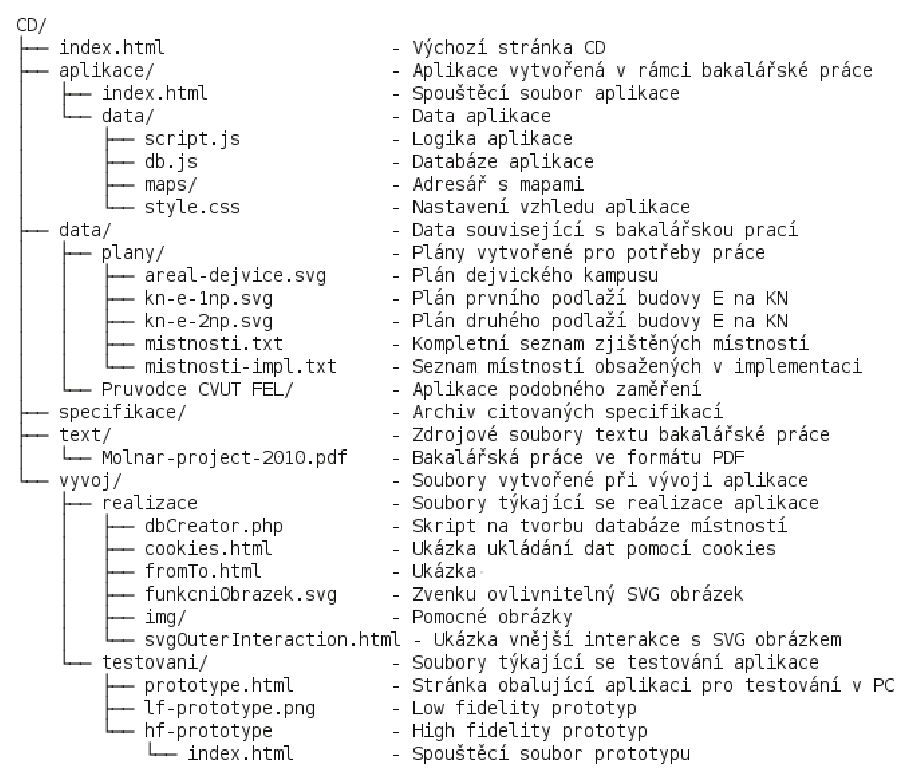
\includegraphics{figures/tree}
% \caption{Struktura přiloženého CD}
% \label{fig:tree}
\end{center}
\end{figure}
